%% myFigures.tex
% A common file to store all figure definitions
%
% In preparing your thesis, one of the first things you should do is
% organize your figures.  Then, one of the last things you'll do is
% reorder your figures so they display where you want them to in the
% text.  Organizing figure definitions in a common files helps:
%
%   1. Write new figures using earlier examples.
%
%   2.  Isolate code and minimize the risk of introducing bugs in the
%   final editing process.  Trust me, moving around just one line of
%   code is easier.
%
%   3.  Reuse figures in other papers.  <=== the best reason!
%
% Note command names can not include numbers and special characters.
%
% To make the file more searchable, use naming conventions that map
% the graphics filename labSetup.jpg to the command name \figlabSetup to the
% figure label fig:labSetup.
% 

\newcommand{\figSmallPatch}{
\begin{figure}[tbp] \centering
\begin{subfigure}{.32\textwidth} \centering
  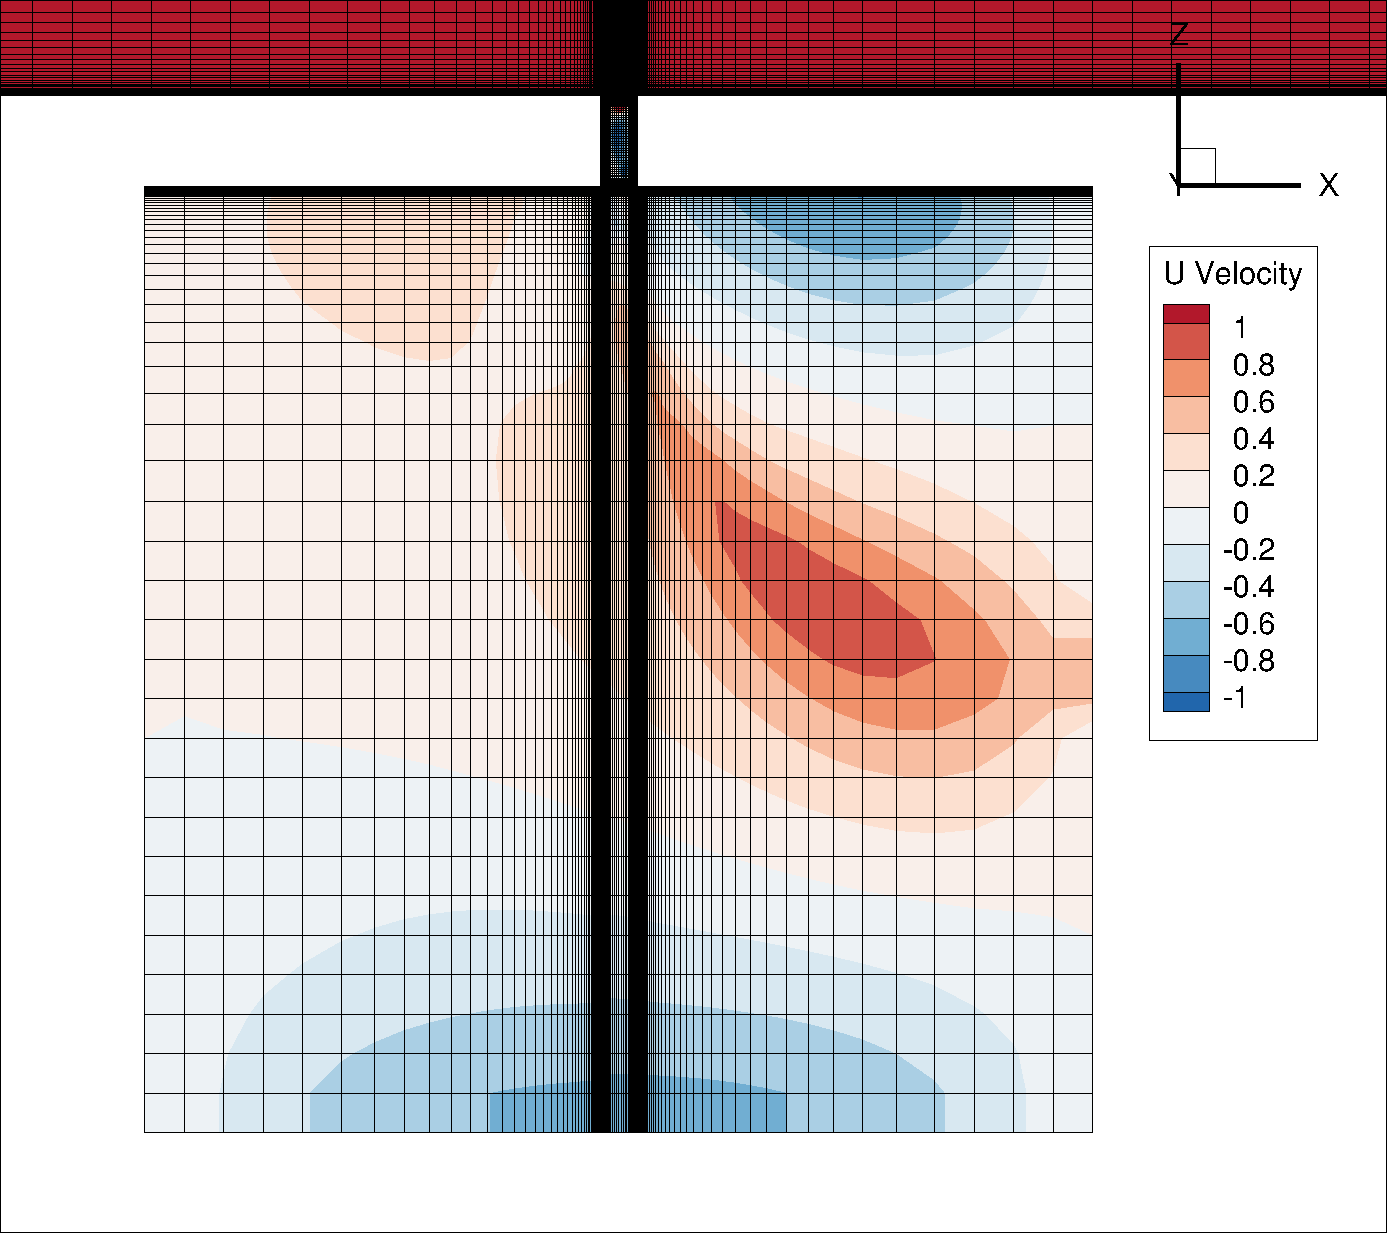
\includegraphics[width=1\linewidth]{1-1_grid.png}
\end{subfigure}%
\begin{subfigure}{.32\textwidth} \centering
  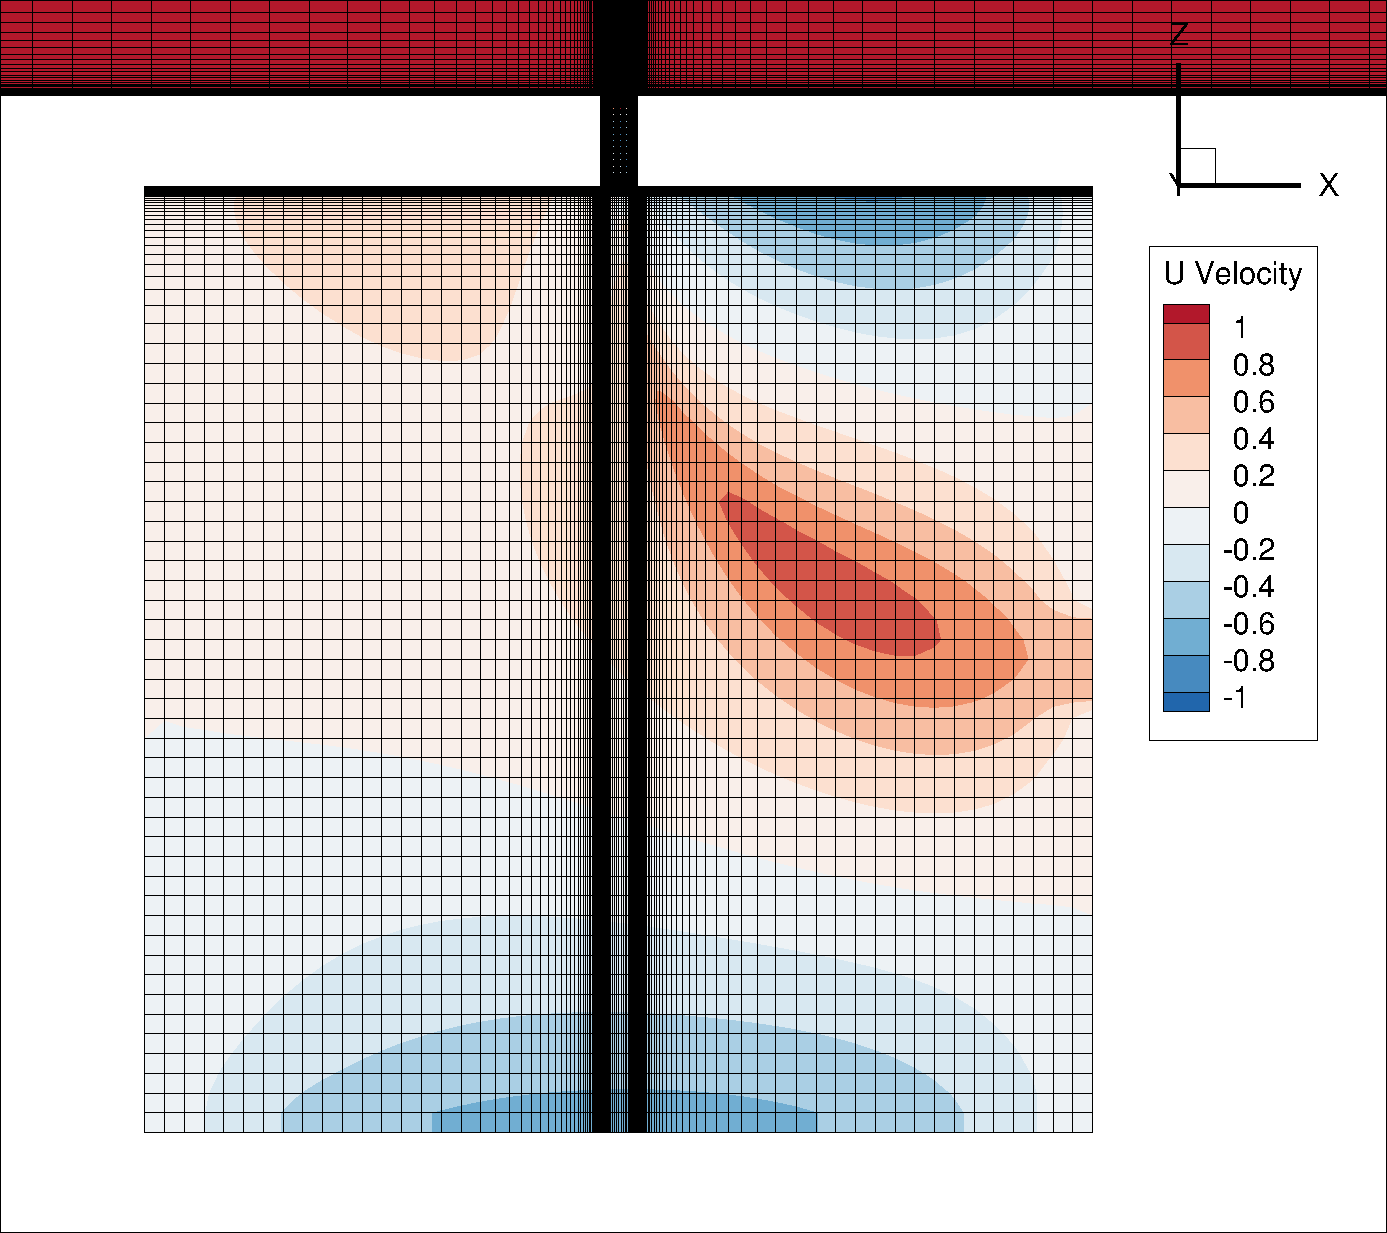
\includegraphics[width=1\linewidth]{1-2_grid.png}
\end{subfigure}%
\begin{subfigure}{.32\textwidth} \centering
  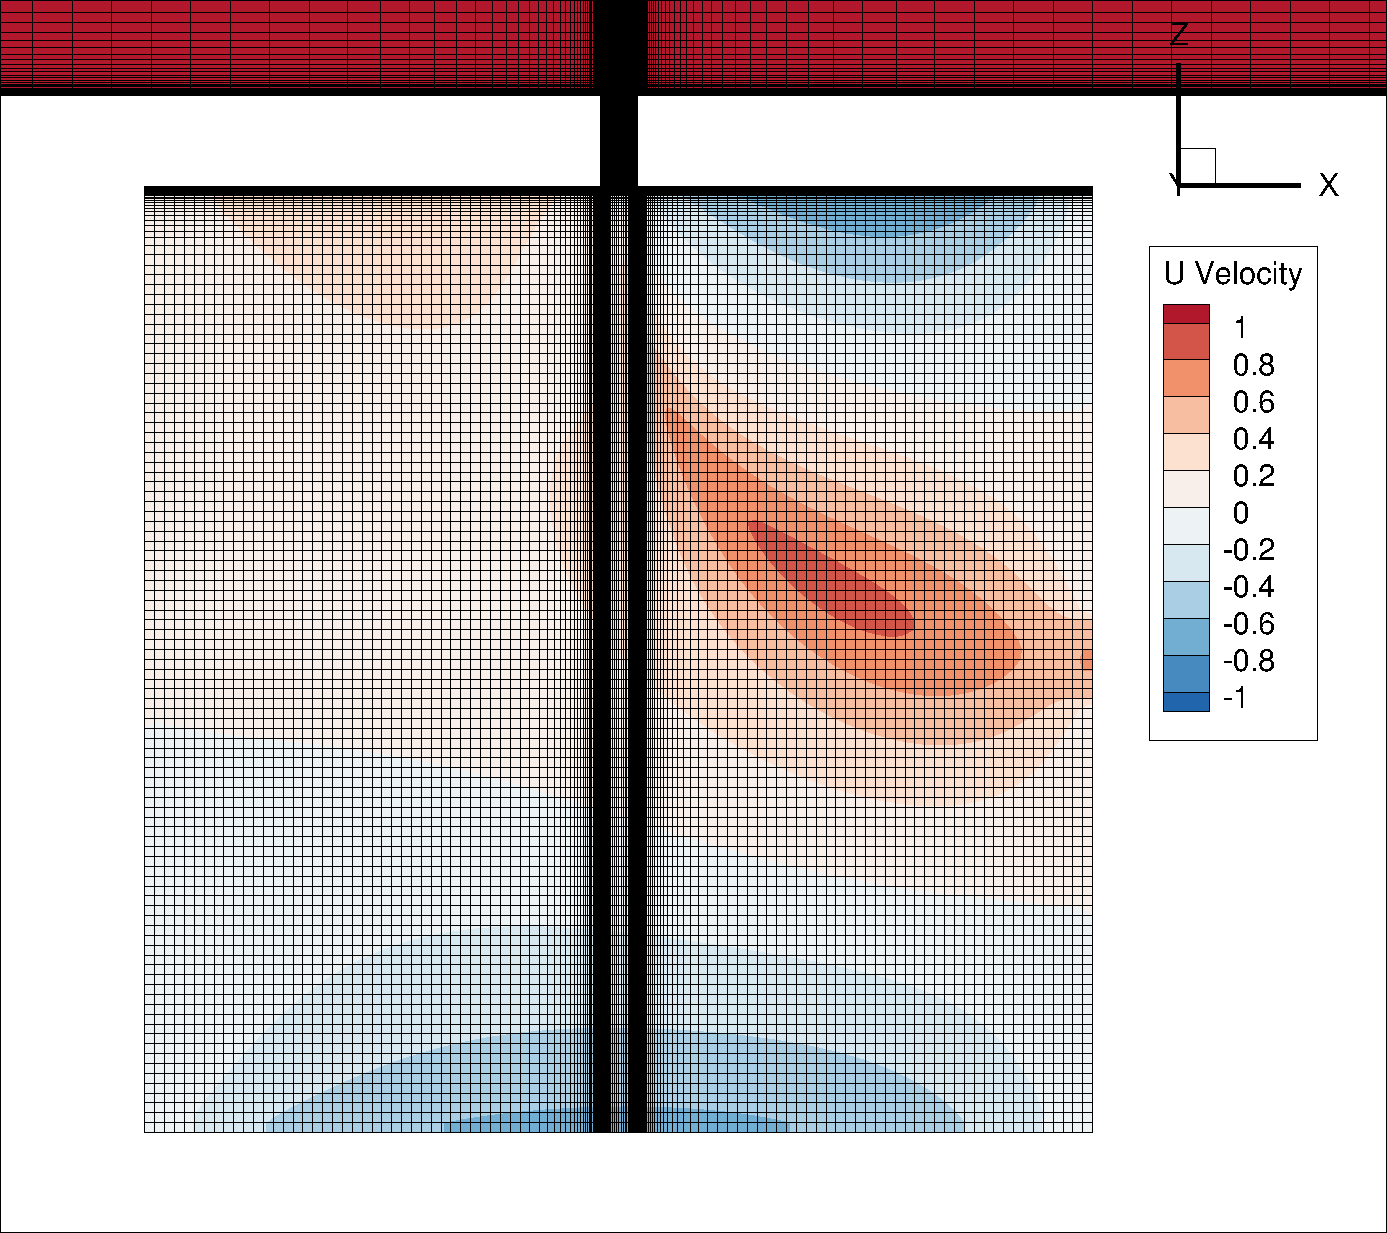
\includegraphics[width=1\linewidth]{1-3_grid.png}
\end{subfigure}
\begin{subfigure}{.32\textwidth} \centering
  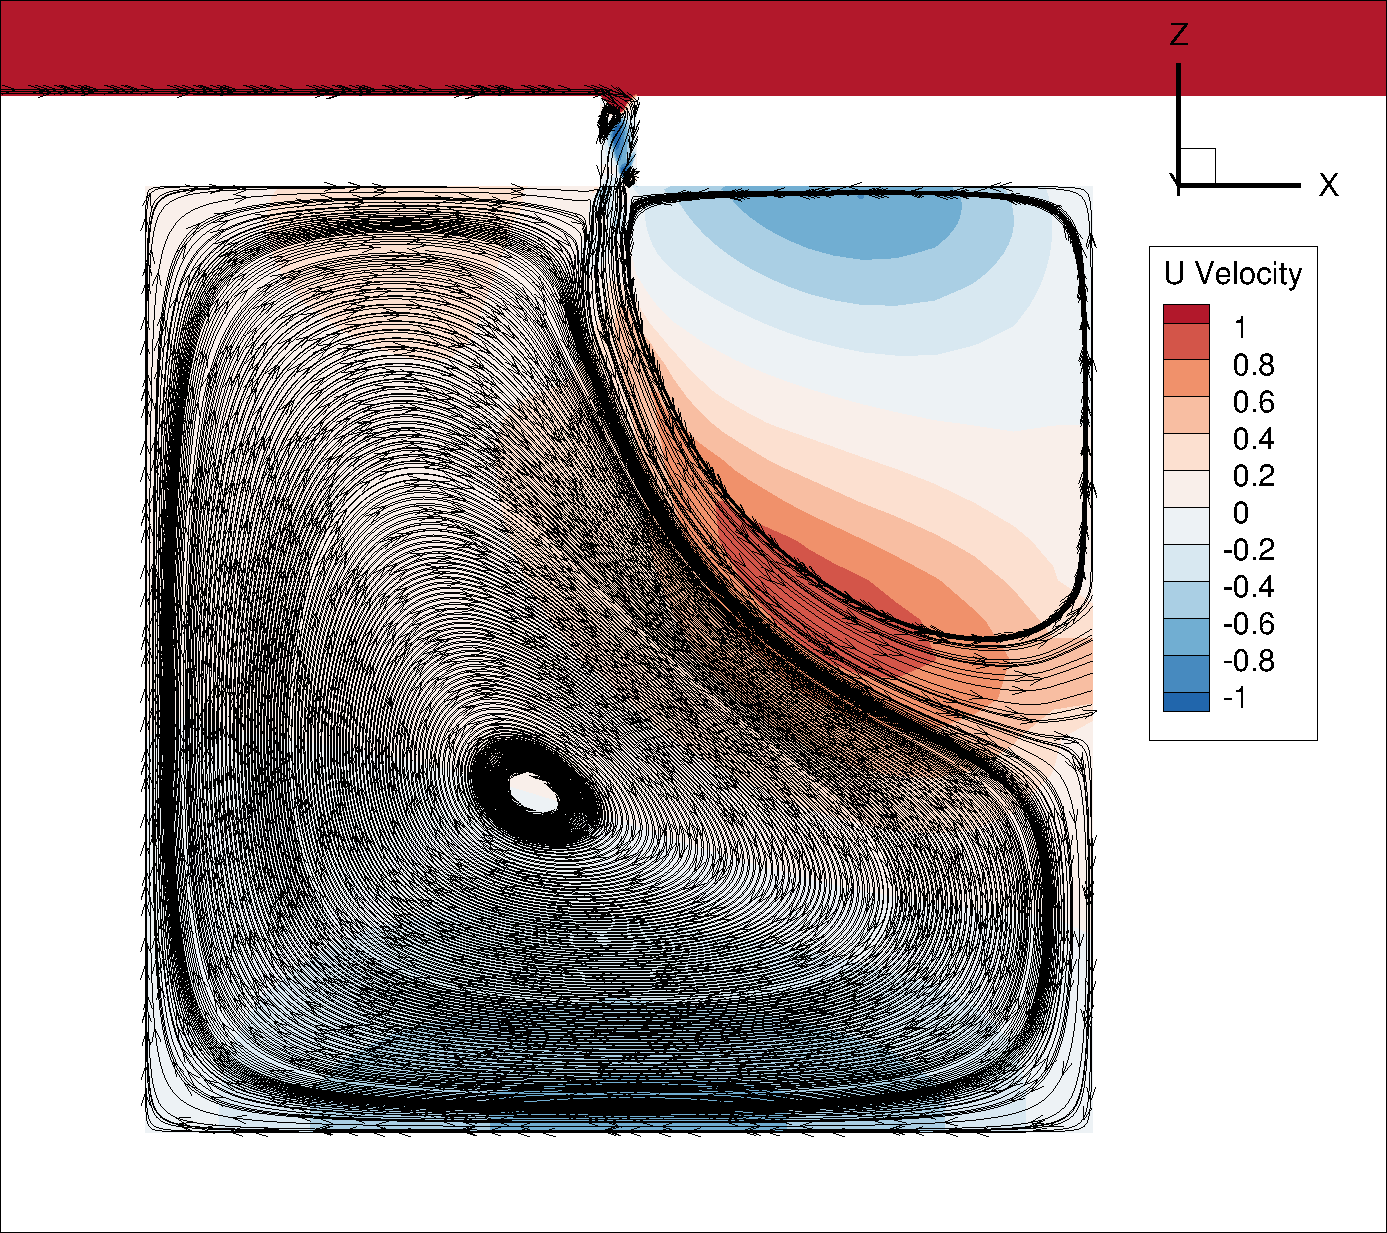
\includegraphics[width=1\linewidth]{1-1_streamlines.png}
\end{subfigure}%
\begin{subfigure}{.32\textwidth} \centering
  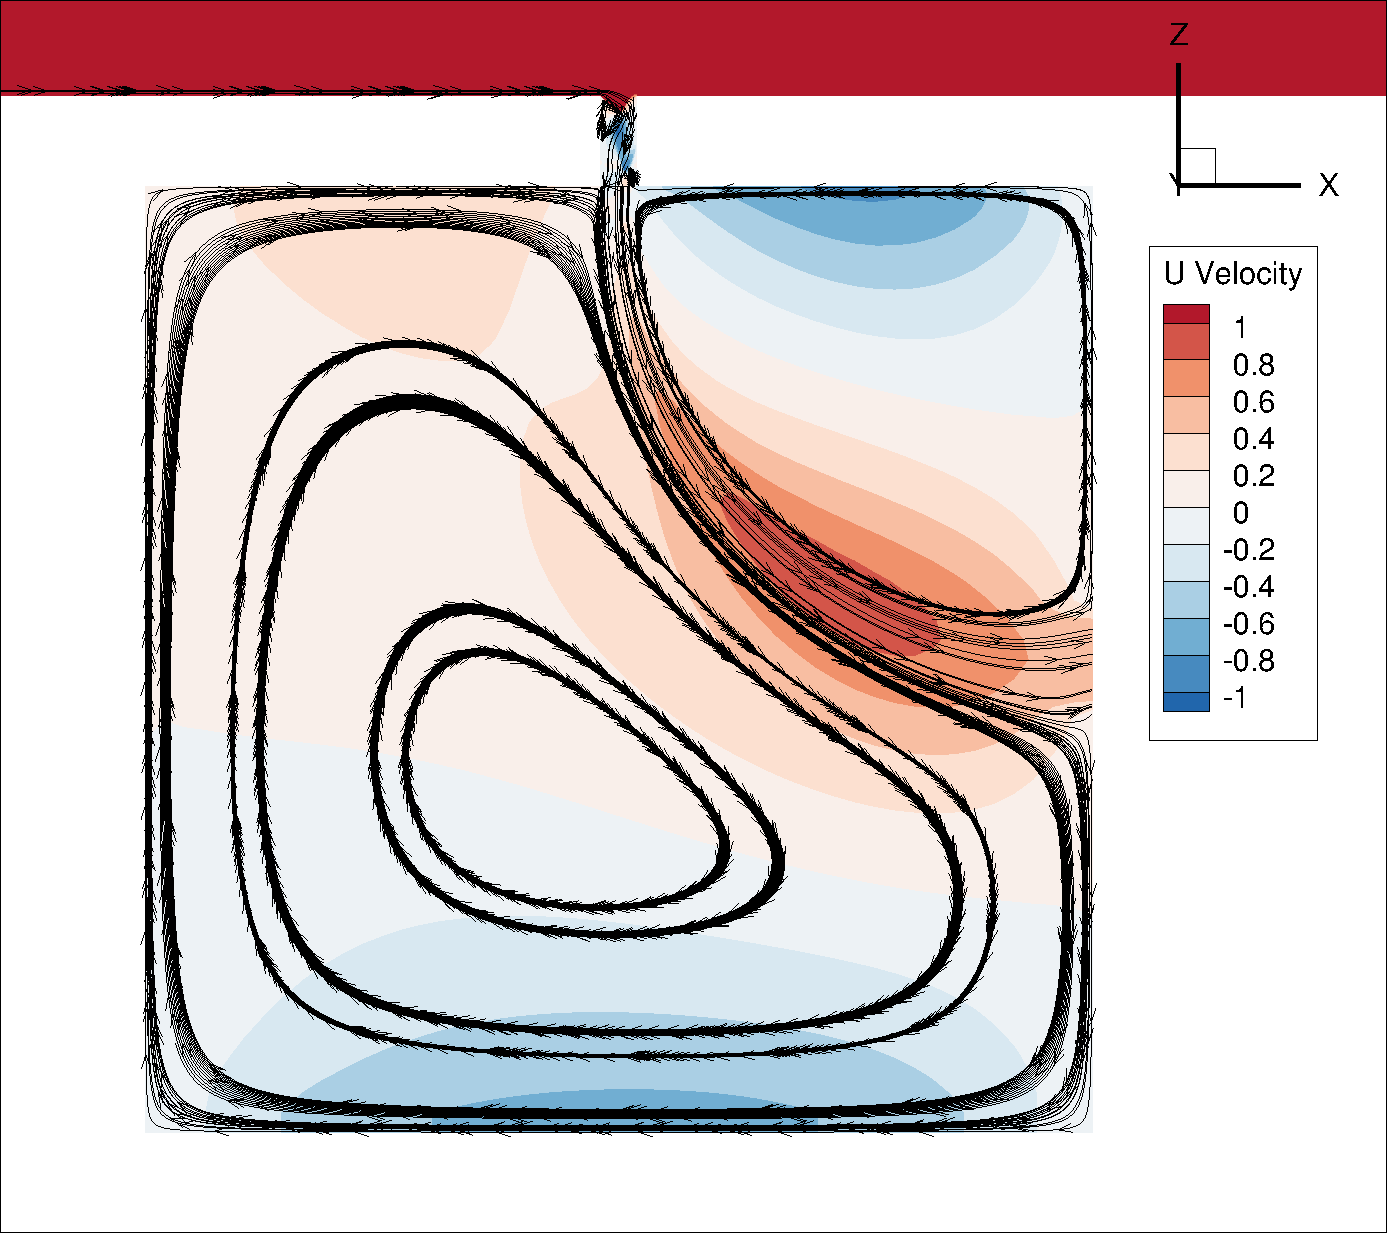
\includegraphics[width=1\linewidth]{1-2_streamlines.png}
\end{subfigure}%
\begin{subfigure}{.32\textwidth} \centering
  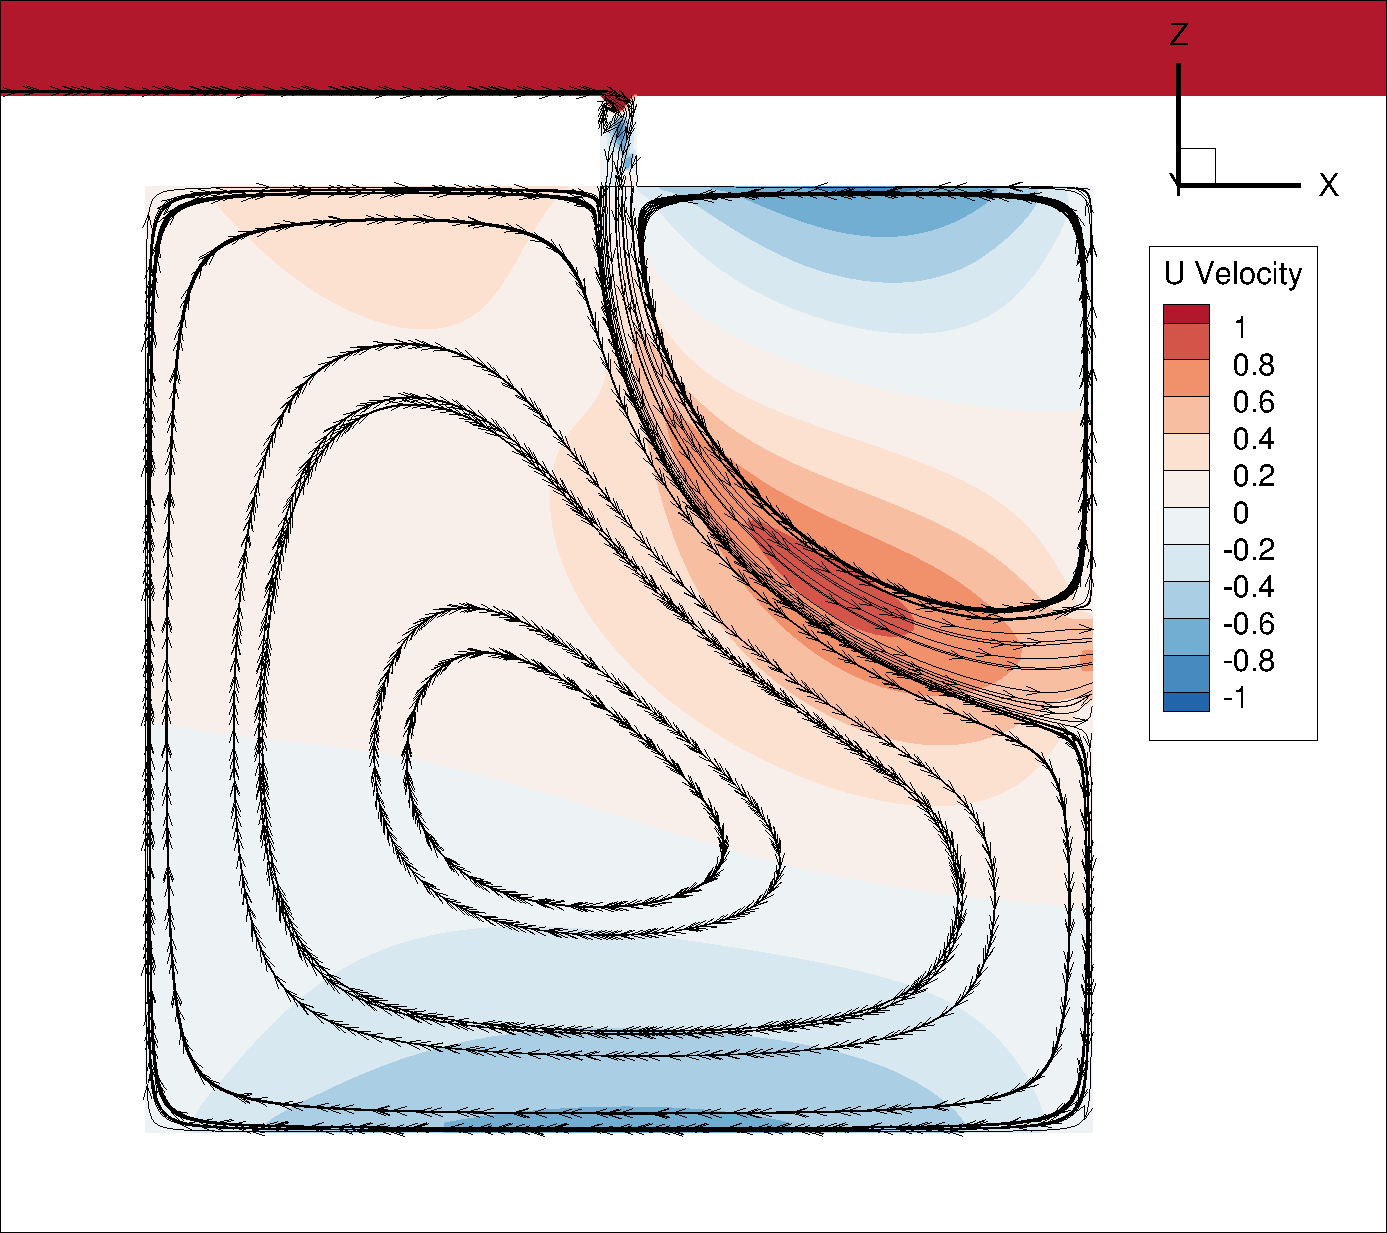
\includegraphics[width=1\linewidth]{1-3_streamlines.png}
\end{subfigure}
  \caption{Grid resolution study of the contours of u-velocity and streamlines for the small patch}
  \label{fig:small}
\end{figure}}
	

\newcommand{\figMeshOverlay}{
\begin{figure}[tbp] \centering
\begin{subfigure}{0.8\textwidth} \centering
  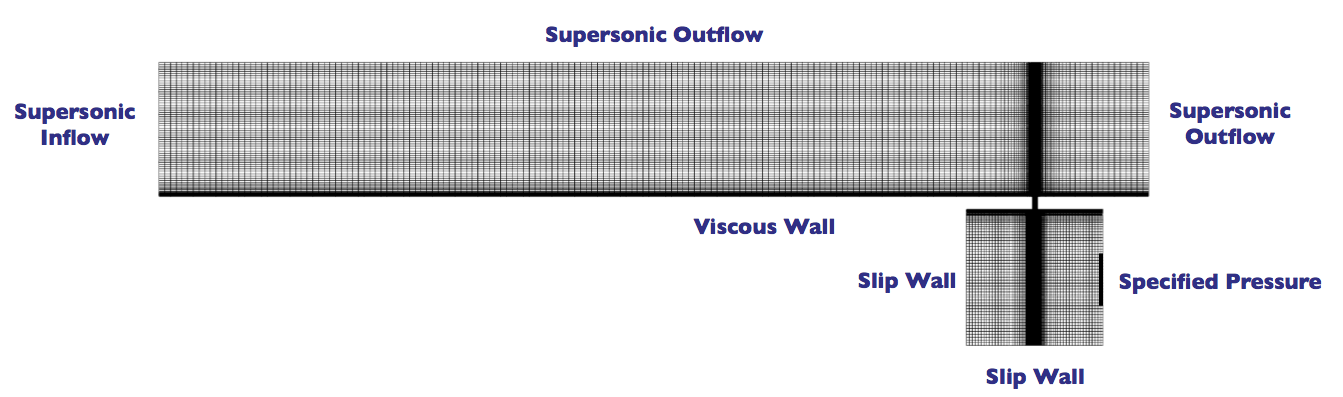
\includegraphics[width=1\linewidth]{mesh.png}
\end{subfigure}
\begin{subfigure}{.65\textwidth} \centering
  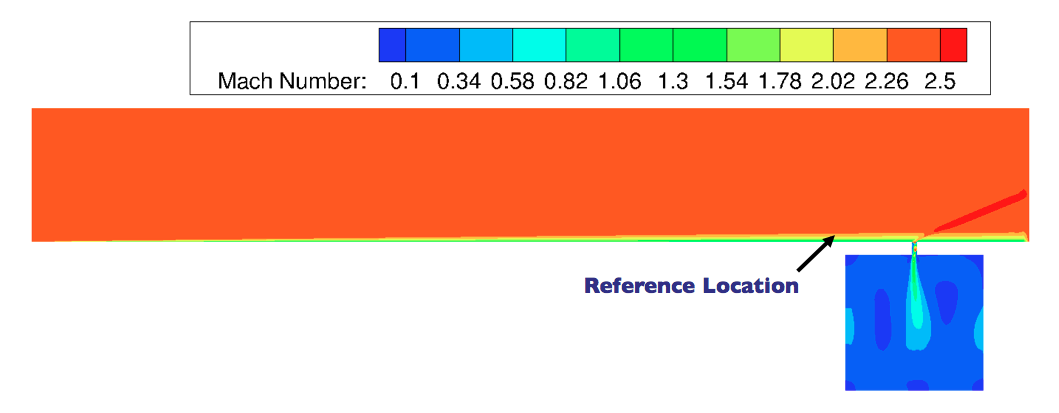
\includegraphics[width=1\linewidth]{overview_solution.png}
\end{subfigure}%
  \caption{Grid setup}
  \label{fig:tun}
\end{figure} }

\newcommand{\figMyFirstLaTeX}{\begin{figure}[tbp]
 \begin{center}
    \includegraphics[width=6in]{myFirstLaTeXCursor}
     \caption[\LaTeX\ a very simple document]{Compile a very simple document.}
     \label{fig:MyFirstLaTeX}
 \end{center}
 \vspace{-0.2 in}
\end{figure}
}

\newcommand{\figafitStyle}{\begin{figure}[tbp]
 \begin{center}
    \includegraphics[width=6in]{myFirstLaTeXafit}
     \caption{Recompile using afitThesis.sty, the AFIT
     thesis style file.}
     \label{fig:afitStyle}
 \end{center}
\end{figure}
}

\newcommand{\figtitlePage}{\begin{figure}[tbp]
 \begin{center}
    \includegraphics[width=6in]{titlePage}
     \caption{Enter student data in titlePage.tex to customize the
     document's first pages.}
     \label{fig:titlePage}
 \end{center}
\end{figure}
}

\newcommand{\figmyFlypage}{\begin{figure}[tbp]
 \begin{center}
    \includegraphics[width=6in]{myFlypage}
     \caption{Here we have compiled the first four page of a thesis.}
     \label{fig:myFlypage}
 \end{center}
\end{figure}
}

\newcommand{\figmyFirstAbstract}{\begin{figure}[tbp]
 \begin{center}
    \includegraphics[width=6in]{myFirstAbstract}
     \caption{Add an abstract to the front matter of your thesis.}
     \label{fig:myFirstAbstract}
 \end{center}
\end{figure}
}

\newcommand{\figmyFigures}{\begin{figure}[tbp]
 \begin{center}
    \includegraphics[width=5in]{myFigures}
     \caption{Consider defining all your figures in one file.}
     \label{fig:myFigures}
 \end{center}
\end{figure}
}


\newcommand{\figmyFirstFigures}{\begin{figure}[tbp]
 \begin{center}
    \includegraphics[width=6in]{myFirstFigures}
     \caption{Add figures in the main matter of your document; fill in
     the document around your graphics.}
     \label{fig:myFirstFigures}
 \end{center}
\end{figure}
}

\newcommand{\figmyFirstBibTeX}{\begin{figure}[tbp]
 \begin{center}
    \includegraphics[width=6in]{myFirstBibTeX}
     \caption{Add your bibliography.}
     \label{fig:myFirstBibTeX}
 \end{center}
\end{figure}
}



